\section{Estado del arte}
	
	El trabajo realizado por \cite{kabeel_performance_2022} hace una investigación sobre la mejora de los mecanismos de transferencia de calor de los destiladores solares, donde se estudia el desempeño de un destilador semiesférico con diferentes tipos de aletas cilíndricas proponiendo diseños como el mostrado en la~\cref{fig:solar-finned-distiller}. Para ver la mejora en el rendimiento, el sistema se probó durante tiempos de 12 horas continuas por 3 días y los resultados obtenidos se compararon contra un destilador semiesférico convencional. 	
		
	\begin{figure}[H]
		\centering
		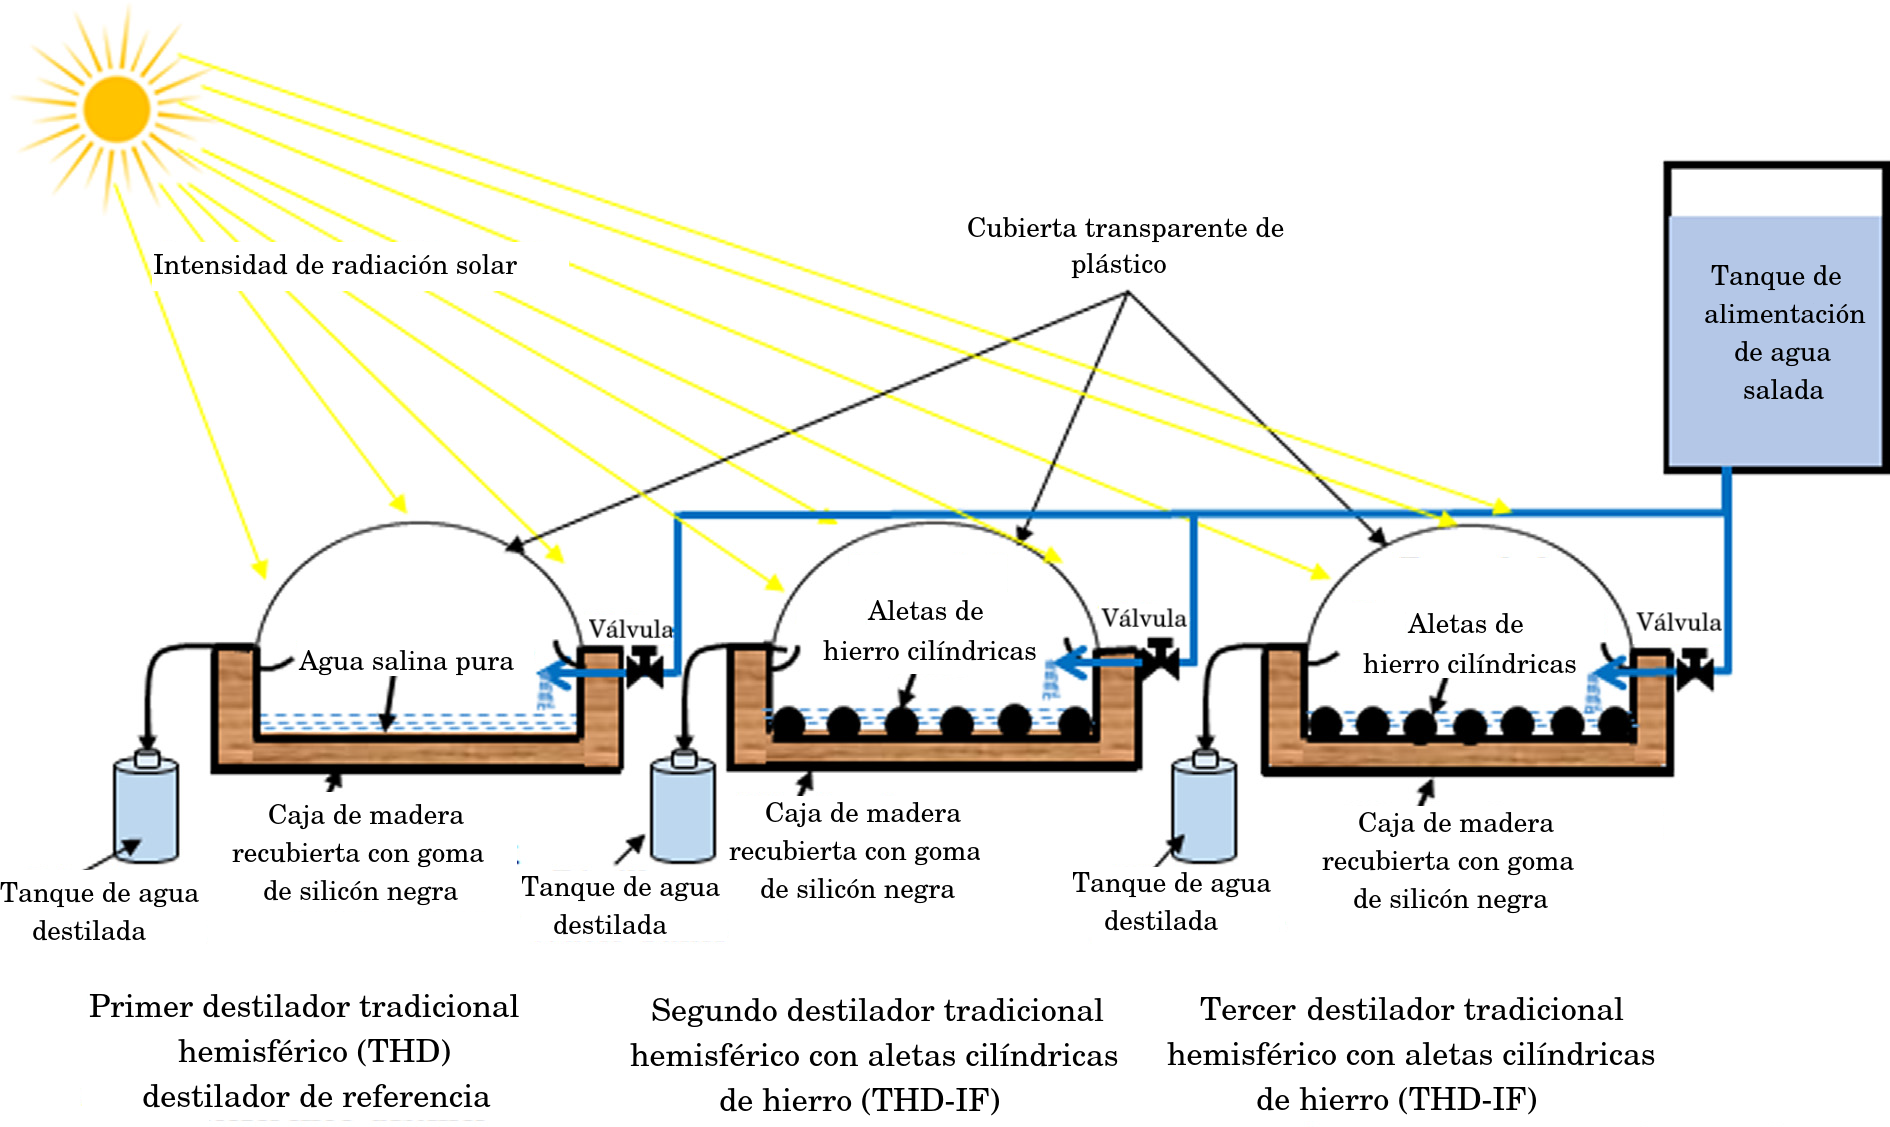
\includegraphics[width=0.8\linewidth, keepaspectratio]{Estado-del-arte/solar-finned-distiller.png}
		\caption{Aletas cilíndricas para mejorar los mecanismos de transferencia de calor de un destilador solar pasivo}
		\floatfoot{Figura obtenida de \cite{kabeel_performance_2022}}
		\label{fig:solar-finned-distiller}
	\end{figure}
	
	De los resultados se observó una mejora de \SI{4.80}{\litre\per\day} del destilador convencional a un promedio de \SI{5.74}{\litre\per\day} del destilador aletado, también se alcanzó una eficiencia de hasta \qty{53.52}{\percent} y se determinó que el sistema tenía una recuperación económica de 24 días.
	
	Jobrane et al. \cite{jobrane_theoretical_2022} propusieton en 2022 un destilador de dos cámaras; se estimó que el costo del agua generada es de 25 euros por cada cien litros de agua, teniendo una producción promedio de \SI{4.03}{\litre\per\m\tothe{2}\day} considerando una potencia recibida promedio de \SI{380}{\watt\per\m\tothe{2}}. Sobre el agua obtenida se realizaron estudios físicos y químicos donde se determinó que poseía buena calidad para beber.
	
	En la~\cref{fig:solar-wick-distiller} se observa la configuración usada; el sistema consta de una cámara de evaporación la cual distribuye el agua bombeada uniformemente sobre una lámina de aluminio AW6060 donde acopla un extractor para forzar la convección del vapor generado hacia la cámara de condensación, donde se reutiliza el calor latente de vaporización para precalentar el agua salobre y a su vez condensar el vapor. Para su alimentación se usó una bomba peristáltica controlada automáticamente y optimizada según el rendimiento visto en el destilador.
	
	\begin{figure}[H]
		\centering
		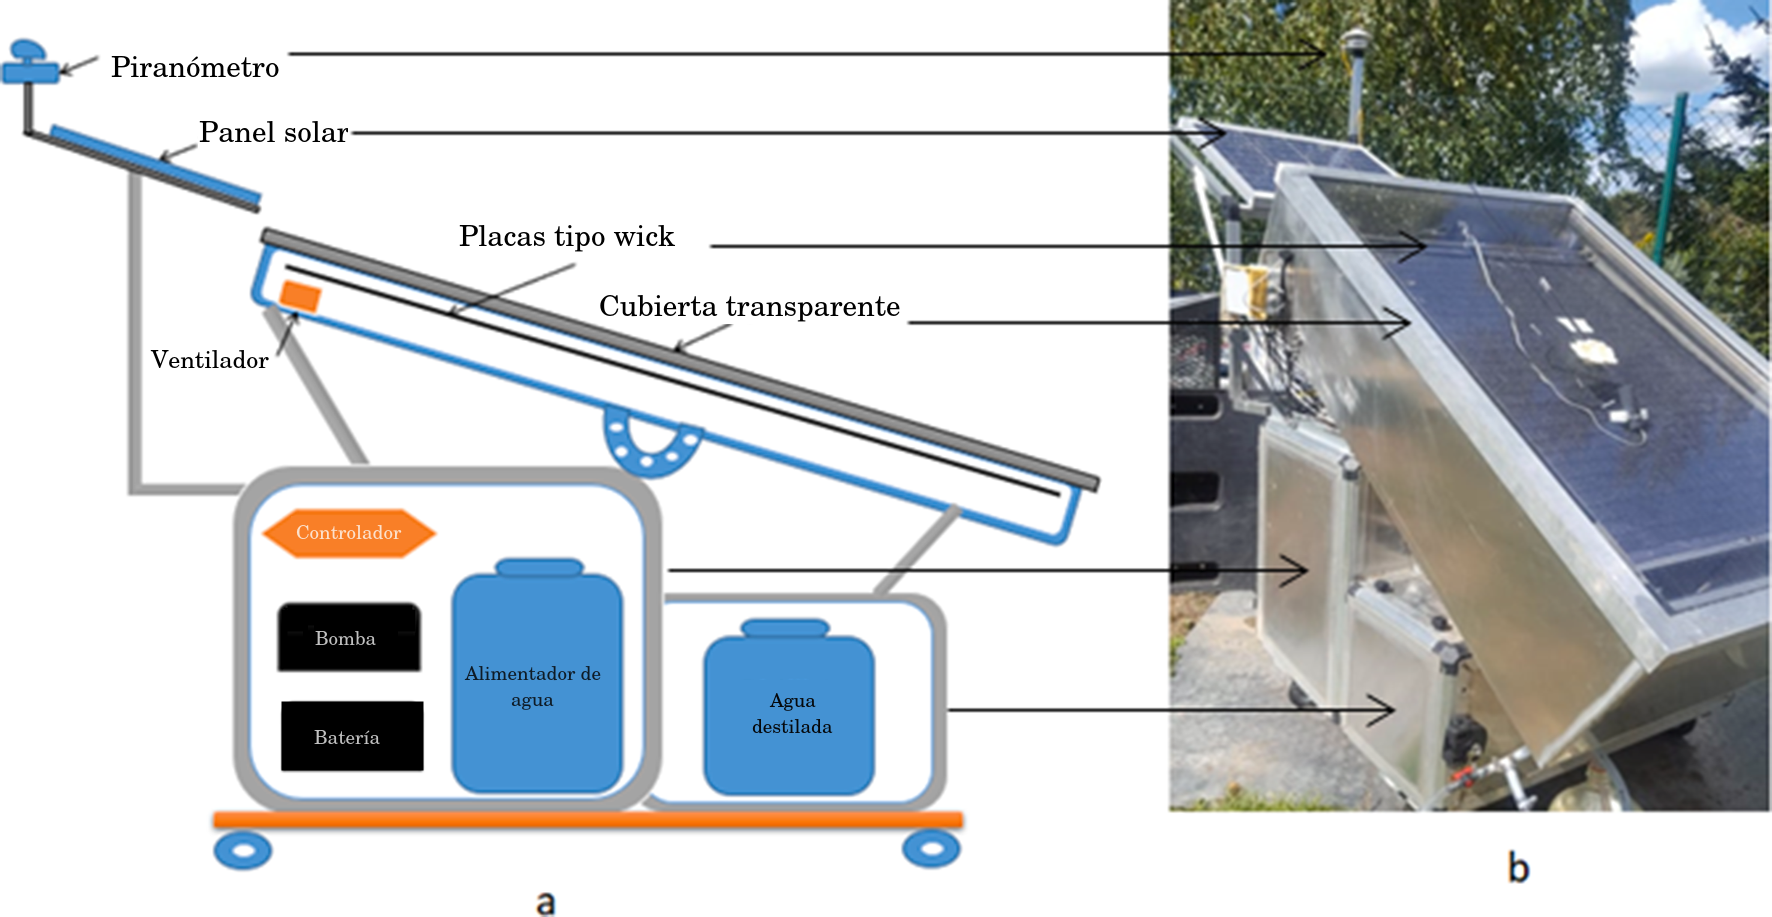
\includegraphics[width=0.8\linewidth, keepaspectratio]{Estado-del-arte/solar-wick-distiller.png}
		\caption{Destilador solar de dos cámaras con ventilador}
		\floatfoot{Figura obtenida de \cite{jobrane_theoretical_2022}}
		\label{fig:solar-wick-distiller}
	\end{figure}
	
	Palomino et al. \cite{palomino-resendiz_design_2018} propusieron un destilador solar híbrido el cual alcanza los \SI{10}{\litre} por día en días soleados con menos de \SI{13}{\gram\per\litre} de sales disueltas. En la \cref{fig:palomino-distiller} se observa el esquema propuesto, el cual se monta sobre una estructura robótica acoplada a un sistema de seguimiento solar y un sistema de control para regular la alimentación del agua. Se observa que este sistema aprovecha tanto la energía solar térmica como la solar fotovoltaica cuyos excedentes son almacenados en baterías.
	
	Este desalinizador totalmente autónomo es potenciado mediante el uso de lentes de Fresnel y un calentador eléctrico. La energía térmica generada por ambos instrumentos es aprovechada dentro de una cámara adiabática de evaporación la cual lleva el vapor generado a un condensador externo.
	
	\begin{figure}[H]
		\centering
		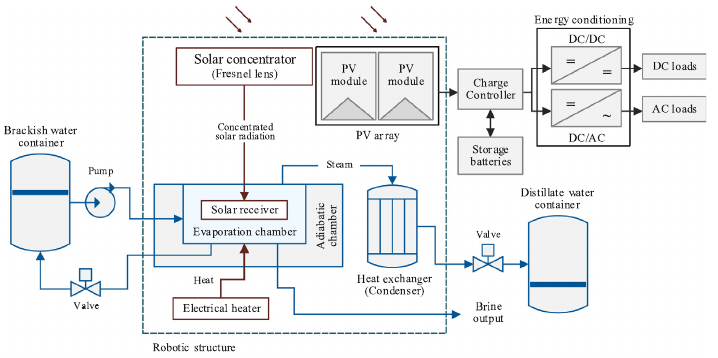
\includegraphics[width=0.8\linewidth, keepaspectratio]{Estado-del-arte/palomino-distiller.png}
		\caption{Destilador solar activo e híbrido con la incorporación de un calentador eléctrico y lentes de concentración.}
		\floatfoot{Figura obtenida de \cite{palomino-resendiz_design_2018}}
		\label{fig:palomino-distiller}
	\end{figure}